\documentclass[12pt]{article}

\usepackage[longnamesfirst]{natbib}
\usepackage{listings}
\usepackage{graphicx}
\usepackage{float}
\usepackage{amsmath}
\usepackage{bm}
\usepackage[font=footnotesize]{caption}
\usepackage{subcaption}
\usepackage[margin=1.25in]{geometry}

\newcommand{\m}[1]{\mathbf{\bm{#1}}}
\newcommand{\R}{I\hspace{-4.4pt}R}



\begin{document}

\begin{large}
\noindent AMS 205B Take-Home Final Exam
\smallskip

\noindent Mickey Warner
\end{large}
\bigskip

\section*{Problem 1}

\subsection*{(a)}

\noindent The likelihood is given by
\begin{align*}
L(\m{y}|\m{x},\alpha,\beta,\omega,\delta,\sigma^2) &= \prod_{i=1}^n(2\pi\sigma^2)^{-1/2}\exp\left\{-\frac{1}{2\sigma^2}[y_i-\alpha-\beta\cos(\omega x_i + \delta)]^2 \right\} \\
 &= (2\pi\sigma^2)^{-n/2}\exp\left\{-\frac{1}{2\sigma^2}\sum_{i=1}^n\left[y_i-\alpha-\beta\cos(\omega x_i + \delta)\right]^2 \right\}
\end{align*}
\noindent If I take the partial derivative w.r.t. $\omega$ of the log-likelihood, we obtain
\[ \frac{\partial}{\partial\omega}\log L &= -\frac{\beta}{\sigma^2}\sum_{i=1}^n(y_i-\alpha-\beta\cos(\omega x_i+\delta))\sin(\omega x_i + \delta)x_i \]
\noindent Thus solving for $\omega$ when this equals 0 has no available closed form. This further means that the m.l.e. for $\theta=(\alpha,\beta,\omega,\delta,\sigma^2)$ is not available in closed form.
\bigskip

\noindent To obtain estimates for the parameters, I use profile likelihoods and iteratively optimize $(\omega, \delta)$ and $(\alpha,\beta,\sigma^2)$ using the \texttt{optim} function in R. The optimization is improved with some reasonable constraints (given our model and data):
\begin{align*}
\alpha &\in (\min_i y_i, \max_i y_i) \\
\beta &\in (\min_i y_i, \max_i y_i) \\
\omega &\in (0, 3) \\
\delta &\in [-\pi, \pi) \\
\sigma^2 &\in (0.001, \mathrm{var}(\m{y}))
\end{align*}
\noindent The estimates are $\hat\theta=(\hat\alpha, \hat\beta, \hat\omega, \hat\delta, \hat\sigma^2)=(1.969, 1.499, 1.752, -0.037, 0.019)$. The $3$ in the bound for $\omega$ is a rough estimate for the maximum number of periods observed in the data. The code is given in the appendix.

\subsection*{(b)}

\noindent To obtain an approximate confidence interval from a Wald-like test, we need to ensure that the regularity conditions are met.
\begin{itemize}
\item A1: our model assumes we have a random sample
\item A2: given the constraint $\delta\in[-\pi,\pi)$, the model is identifiable
\item A3: the parameters do not determine the support
\item A4: there may be a concern if $\delta=-\pi$, but we could just as easily defined $\delta\in[0,\pi)$ to avoid this, so the parameter space contains an open set around the true parameters
\item A5: the normal density is infinitely differentiable as is the function $\cos(\omega x_i+\delta)$ and the derivatives are continuous.
\item A6: though I don't calculate the third derivative of the $\log$, based on the second derivative, shown next,
\end{itemize}
\noindent The Wald approximations for $\omega$ and $\delta$ are given by
\[ \frac{\hat\omega - \omega}{1/\sqrt{I(\hat\omega)}} \sim N(0,1), ~~~~~
    \frac{\hat\delta - \delta}{1/\sqrt{I(\hat\delta)}} \sim N(0,1) \]
\noindent where $\hat\omega$ and $\hat\omega$ are the mles from above,
\begin{align*}
I(\hat\omega) &= \left.-\frac{\partial^2}{\partial\omega^2}\log L(\m{y}|\m{x},\alpha,\beta,\omega,\delta,\sigma^2)\right\vert_{\theta=\hat\theta} \\
&= \left.\frac{\beta}{\sigma^2}\sum_{i=1}^n\left([y_i-\alpha-\beta\cos(\omega x_i+\delta)]\cos(\omega x_i+\delta)x_i^2 + [\beta x_i^2\sin(\omega x_i+\delta)^2]\right)\right\vert_{\theta=\hat\theta} \\
&= 281704.5
\end{align*}
\noindent and,
\begin{align*}
I(\hat\delta) &= \left.-\frac{\partial^2}{\partial\delta^2}\log L(\m{y}|\m{x},\alpha,\beta,\omega,\delta,\sigma^2)\right\vert_{\theta=\hat\theta} \\
&= \left.\frac{\beta}{\sigma^2}\sum_{i=1}^n\left([y_i-\alpha-\beta\cos(\omega x_i+\delta)]\cos(\omega x_i+\delta) + [\beta\sin(\omega x_i+\delta)^2]\right)\right\vert_{\theta=\hat\theta} \\
&= 5397.7.
\end{align*}
\noindent These lead to the following $95\%$ confidence intervals
\begin{align*}
\{\omega : \hat\omega - 1/\sqrt{I(\hat\omega)} z_{0.975} < \omega < \hat\omega + 1/\sqrt{I(\hat\omega)} z_{0.975} \} &= (1.748, 1.756) \\
\{\delta : \hat\delta - 1/\sqrt{I(\hat\delta)} z_{0.975} < \delta < \hat\delta + 1/\sqrt{I(\hat\delta)} z_{0.975} \} &= (-0.063, -0.010)
\end{align*}

\subsection*{(c)}

\noindent The parametric bootstrap procedure yields the confidence intervals
\begin{align*}
\omega &\in (1.745, 1.760) \\
\delta &\in (-0.092, 0.016) 
\end{align*}
\noindent which are wider than those based on the normal approximation.

\subsection*{(d)}

\noindent I would test $H_0:\delta=0$ versus $H_a:\delta\neq 0$ based on the confidence interval from the bootstrap sample since this will be closer to the exact interval than the approximation would be. Since 0 is contained the interval, we do not have enough evidence to reject the null that $\delta=0$. 
 
\section*{Problem 2}

\subsection*{(a)}

\noindent The likelihood is
\[ L\equiv L(\m{x},\m{y}|\lambda_1,\lambda_2) = \lambda_1^{-n}\lambda_2^{-n}e^{-\sum x_i / \lambda_1}e^{-\sum y_i / \lambda_2} \]
\noindent The unconstrained maximum is found by taking the derivative of the log-likelihood and setting it equal to 0.
\begin{align*}
\frac{\partial}{\partial \lambda_1} \log L = -\frac{n}{\lambda_1} + \frac{1}{\lambda_1^2}\sum x_i \overset{set}= 0 \\
\hat\lambda_1 = \bar x
\end{align*}
\noindent The second derivative evaluated at $\lambda_1=\hat\lambda_1$ gives
\[ \left.\frac{\partial^2}{\partial \lambda_1^2} \log L \right\vert_{\lambda=\bar x} = \frac{n}{(\bar x)^2} - \frac{2}{(\bar x)^3}\sum x_i = -\frac{n^3}{(\sum x_i)^2} < 0\]
\noindent so we have a maximum. By similar logic, $\hat\lambda_2 = \bar y$.
\bigskip

\noindent Under the null hypothesis, the maximum depends on $\bar x$ and $\bar y$. If $\bar x \leq \bar y$, then the constrained maximum occurs at the same location as the unconstrained. For the case $\bar x > \bar y$, we must check along the border $\lambda_1=\lambda_2$. The other boundaries are not of interest since $L$ will be increasing toward $\lambda_1=\lambda_2$.
\bigskip

\noindent The mle under the constrained likelihood solves the equation
\begin{align*}
\frac{\partial}{\partial \lambda}\log L(\m{x},\m{y}|\lambda_1=\lambda,\lambda_2=\lambda) &= -\frac{2n}{\lambda} + \frac{1}{\lambda^2}\left(\sum x_i + \sum y_i\right) \overset{set}= 0 \\
\Rightarrow \hat\lambda &= \frac{\sum x_i + \sum y_i}{2n}
\end{align*}
\noindent The likelihood ratio is then given by
\begin{align*}
\kappa \equiv LRT &= \begin{cases} 1 & \bar x \leq \bar y \\ \frac{\sup_{\lambda_1\leq\lambda_2}L(\m{x},\m{y}|\lambda_1,\lambda_2)}{\sup_{\lambda_1,\lambda_2}L(\m{x},\m{y}|\lambda_1,\lambda_2)} & \bar x > \bar y \end{cases} \\
&= \begin{cases} 1 & \bar x \leq \bar y \\ \frac{(\bar x \bar y)^n}{[\frac{1}{2}(\bar x + \bar y)]^{2n}} & \bar x > \bar y \end{cases} \\
\end{align*}
\noindent We reject null when $\kappa<c$ for some constant $0<c<1$. We will reject only if $\bar x > \bar y$, so this is the case we're interested in. We simplify the rejection region
\begin{align*}
R = \left\{(x,y):\frac{(\bar x\bar y)^n}{[\frac{1}{2}(\bar x + \bar y)]^{2n}} < c \right\} &= \left\{(x,y):\frac{\bar x\bar y}{(\bar x + \bar y)^2} < c \right\}  \\
&= \left\{(x,y):\frac{(\bar x + \bar y)^2}{\bar x \bar y} > c \right\}  \\
&= \left\{(x,y):\frac{\bar x^2 + 2\bar x\bar y + \bar y^2}{\bar x \bar y} > c \right\}  \\
&= \left\{(x,y):\frac{\bar x}{\bar y} + \frac{\bar y}{\bar x}+2 > c \right\}  \\
&= \left\{(x,y):\frac{\sum x_i}{\sum y_i} + \frac{\sum y_i}{\sum x_i}+2 > c_\alpha \right\}
\end{align*}
\noindent where $c_\alpha$ is chosen so $Pr((\m{x},\m{y})\in R|\lambda_1\leq\lambda_2)=\alpha$. The exact $p$-value is 
\[ Pr\left(\frac{\sum x_i}{\sum y_i} + \frac{\sum y_i}{\sum x_i}+2 > c_\alpha;\lambda_1\leq\lambda_2\right) \]
\noindent It was at this point that I started thinking I was doing everything wrong. I have no idea how to compute this correctly. The closest I got is some gamma-looking distribution. I tried showing that we could reject if $\sum x_i + \sum y_i$ is high, but couldn't figure that out.

\subsection*{(b)}

\noindent Since we're working with the exponential distribution, the regularity conditions are met and a Wald test for the statistic $T=\bar X - \bar Y$ can be given by
\[ Z = \frac{\bar X - \bar Y}{1/\sqrt{I(\hat\lambda)}} \sim N(0,1) \]
\noindent where $I(\hat\lambda)$ is the observed information number under the null (or rather, for $\lambda_1=\lambda_2$). Again, something seemed wrong, especially given the $p$-values I calculated.

\subsection*{(c)}

\noindent Under the null, the observations from both samples can be re-arranged in any order. We combine the $x_i$'s and $y_i$'s into a single vector, then randomly permute the elements. This first $n$ are treated as the $x_i$'s and the last $n$ the $y_i$'s.  We then compute the (permuted) statistic $\bar x - \bar y$ of the permuted sample. We do this many times and store all of the statistics from the permuted sample. We can then compute a $p$-value by counting how many of the permuted statistics were larger than our observed and divide by the number of permutations made.

\subsection*{(d)}

\noindent I wasn't able to get a definitive $p$-value for (a). My attempts gave varied results.
\bigskip

\noindent For (b), I calculated $p_B=0.000389$, which seems outrageously small.
\bigskip

\noindent For (c), I got $p_C=0.037$ which seems reasonable. Assuming I did anything right (which is doubtful), the $p$-values do not agree. I would learn toward $p_C$ being the most correct, though it may be off since I didn't do all possible permutations. My conclusion would be that $\lambda_1>\lambda_2$, but what do I know.


\section*{Problem 3}

\subsection*{(a)}

\noindent The power function is
\begin{align*}
\beta_1(\theta) &= P\left(\sqrt{n}\frac{(\bar X - \theta_0)}{S} > c_1\right) \\
    &= P\left(\sqrt{n}\frac{(\bar X - \theta)}{S} > c_1 + \sqrt{n}\frac{(\theta_0-\theta)}{S}\right) \\
    &= P\left(T_{n-1} > c_1 - \sqrt{n}\frac{(\theta-\theta_0)}{S}\right)
\end{align*}
\noindent where $T_{n-1}$ is a $t$ random variable with $n-1$ degrees of freedom and $c_1$ is chosen such that $\beta_1(\theta_0)=P(T_{n-1} > c_1) = \alpha$.

\subsection*{(b)}

\noindent Assuming $T=\sqrt{n}(\bar X - \theta_0)/S$ follows a standard normal under the null hypothesis, an approximate power function is
\begin{align*}
\beta_2(\theta) &= P\left(Z > c_2 - \sqrt{n}\frac{(\theta-\theta_0)}{S}\right)
\end{align*}
\noindent where $c_2$ satisfies $\beta_2(\theta_0)=P(Z>c_2)=\alpha$. For $T$ to be normal under the null, this would seem to imply $T$ is also normal for $\theta > \theta_0$ (given our sample population).

\subsection*{(c)}

\noindent Figure 1 shows graphs for $\beta_1(\theta)$ and $\beta_2(\theta)$ at $n=10,n=100$,and $n=1000$. As $n$ increases, the power increases, notably for $\theta$ close to $\theta_0$. This makes sense because if the true $\theta$ is different than $\theta_0$, however small, we'd expect to have more power in our test as the sample size increases. Also, $\beta_2$ is greater than $\beta_1$ for all $\theta$.

\subsection*{(d)}

\noindent I think the LRT could shown to reject for small values and since the hypotheses could be written as union-intersection tests, Theorem 8.3.21 could apply leaving us $\beta_2(\theta)$ as most powerful.

\subsection*{(e)}

\noindent I take ``true standard deviation of the data'' to mean $S$. I think it should be $\sigma$, but based on my power functions, the correct things don't cancel. We need to find $n$ that satisfies
\[ P(Z > c_2) = \alpha~\mathrm{and}~ \beta_2(\theta_0+2S)=P\left(Z > c_1 -\sqrt{n}\frac{(\theta_0+2S-\theta_0)}{S}\right)=0.8 \]
\noindent For $\alpha=0.05$, $c_2=1.644$. This leaves us with $0.8 &= P\left(Z>1.644 - 2\sqrt{n}\right)$. Since $P(Z>-0.8416)=0.8$, $1.644-2\sqrt{n}=-0.8416$ implies $n=1.545$, but we choose it to be the next largest integer so $n=2$.

\begin{figure}
\begin{center}
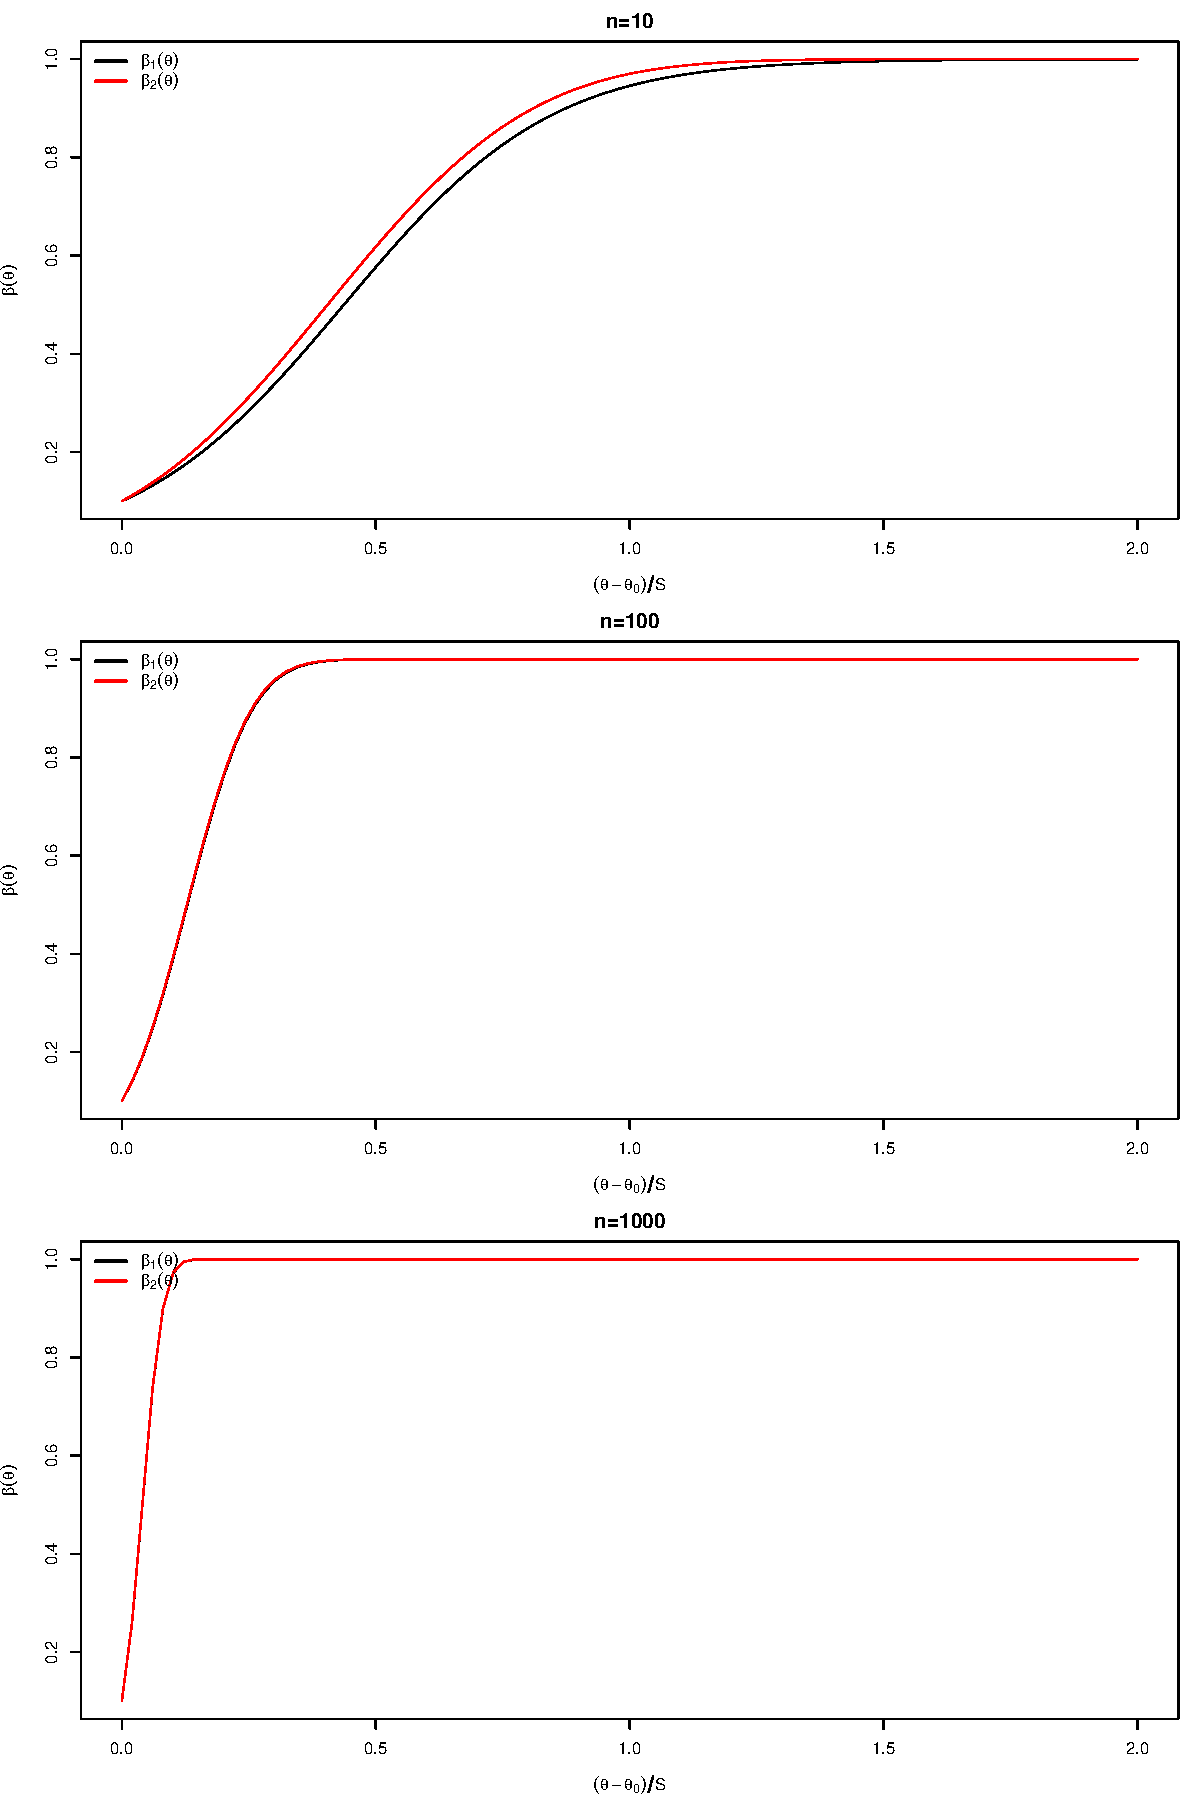
\includegraphics[scale=0.6]{power.pdf}
\caption{Graphs for the two power functions given three different sample sizes.}
\end{center}
\end{figure}

\newpage

\section*{Some of the R code}

\begin{tiny}
\begin{verbatim}
orbits = read.table("~/files/data/205b/orbits.txt", header = TRUE)
n = NROW(orbits)

f1 = function(p, log = TRUE){
    alpha = p[1]
    beta = p[2]
    sig2 = p[3]
    out = -n/2 * log(2*pi*sig2) - 1/(2*sig2)*sum((orbits$Y - alpha -
        beta*cos(omega.hat * orbits$X + delta.hat))^2)
    if (log)
        return (out)
    return (exp(out))
    }
f2 = function(p, log = TRUE){
    omega = p[1]
    delta = p[2]
    out = -n/2 * log(2*pi*sig2.hat) - 1/(2*sig2.hat)*sum((orbits$Y - alpha.hat -
        beta.hat*cos(omega * orbits$X + delta))^2)
    if (log)
        return (out)
    return (exp(out))
    }
f3 = function(p, log = TRUE){
    alpha = p[1]
    beta = p[2]
    omega = p[3]
    delta = p[4]
    sig2 = p[5]
    out = -n/2 * log(2*pi*sig2) - 1/(2*sig2)*sum((orbits$Y - alpha -
        beta*cos(omega * orbits$X + delta))^2)
    if (log)
        return (out)
    return (exp(out))
    }

### (a)
### Profile likelihood
# Initial values for the "fixed" parameters
alpha.hat = mean(c(range(orbits$Y)))    # Estimate for the intercept 
beta.hat = diff(range(orbits$Y))/2      # Estimate for amplitude
sig2.hat = 0.1                          # Guess for variance

# The starting values for the optimizer
xy.1 = expand.grid(
    mean(c(range(orbits$Y))) + seq(-0.2, 0.2, length = 10),
    diff(range(orbits$Y))/2 + seq(-0.2, 0.2, length = 10),
    seq(0.005, 0.1, length = 10))
xy.2 = expand.grid(seq(0, 3, length = 40), seq(-pi, pi, length = 40))

# Iterate through the optimization 5 times (though only 2 may be really necessary)
for (j in 1:5){
    temp.2 = Inf
    for (i in 1:nrow(xy.2)){
        # Optimize treating alpha, beta, sig^2 as fixed (i.e. using alpha.hat,
        # beta.hat, and sig2.hat as the fixed values)
        temp = optim(as.double(xy.2[i,]), function(x) -f2(x, log = TRUE),
            method = "L-BFGS-B", lower = c(0, -pi), upper = c(3, pi))
        # If the i'th starting points produced a better mode, update the parameters
        if (temp$value < temp.2){
            temp.2 = temp$value
            omega.hat = temp$par[1]
            delta.hat = temp$par[2]
            }
        }
    temp.2 = Inf
    for (i in 1:nrow(xy.1)){
        # Optimize treating omega, delta as fixed (using omega.hat and delta.hat)
        temp = optim(as.double(xy.1[i,]), function(x) -f1(x, log = TRUE),
            method = "L-BFGS-B", lower = c(min(orbits$Y), min(orbits$Y), 0.001),
            upper = c(max(orbits$Y), max(orbits$Y), var(orbits$Y)))
        # If the i'th starting points produced a better mode, update the parameters
        if (temp$value < temp.2){
            temp.2 = temp$value
            alpha.hat = temp$par[1]
            beta.hat = temp$par[2]
            sig2.hat = temp$par[3]
            }
        }
    }

### (b)
### Wald-like
I.omega = beta.hat / sig2.hat * sum(
    ((orbits$Y - alpha.hat - beta.hat*cos(omega.hat*orbits$X + delta.hat)) *
    cos(omega.hat*orbits$X + delta.hat)*orbits$X^2) +
    (beta.hat * orbits$X^2 * sin(omega.hat * orbits$X + delta.hat)^2))

I.delta = beta.hat /sig2.hat * sum(
    ((orbits$Y - alpha.hat - beta.hat*cos(omega.hat*orbits$X + delta.hat)) *
    cos(omega.hat * orbits$X + delta.hat)) +
    beta.hat*sin(omega.hat*orbits$X + delta.hat)^2)

# Approx conf int for omega and delta
omega.hat + 1/sqrt(I.omega) * qnorm(0.975) * c(-1, 1)
delta.hat + 1/sqrt(I.delta) * qnorm(0.975) * c(-1, 1)

### (c)
### Bootstrap confidence intervals
B = 5000
boot.par = matrix(0, B, 2) # 2 columns for omega and delta
for (b in 1:B){
    # Generate a bootstrap sample (replace orbits$Y because of how I coded f3)
    orbits$Y = rnorm(n, alpha.hat + beta.hat * cos(omega.hat * orbits$X + delta.hat),
        sqrt(sig2.hat))
    # Compute mles for the bootstrap sample, with the actual mles as starting points
    # Not doing the iterative profile likelihood as before since it takes too long
    # and we are already near the correct values so there shouldn't be any issues
    temp = optim(c(alpha.hat, beta.hat, omega.hat, delta.hat, sig2.hat),
        function(x) -f3(x, log = TRUE), method = "L-BFGS-B",
        lower = c(min(orbits$Y), min(orbits$Y), 0, -pi, 0.001),
        upper = c(max(orbits$Y), max(orbits$Y), 3, pi, var(orbits$Y)))
    boot.par[b,] = temp$par[c(3,4)]
    }

# Comparison
rbind(omega.hat + 1/sqrt(I.omega) * qnorm(0.975) * c(-1, 1),
    quantile(boot.par[,1], c(0.025, 0.975)))

rbind(delta.hat + 1/sqrt(I.delta) * qnorm(0.975) * c(-1, 1),
    quantile(boot.par[,2], c(0.025, 0.975)))


### Problem 2
### (b)
life = read.table("~/files/data/205b/lifetime.txt", header = TRUE)
n = nrow(life)
tobs = mean(life$x) - mean(life$y)
lhat = 0.5*(mean(life$x) + mean(life$y))
I.lambda = -(2*n/(lhat^2) - 2/(lhat^3) * (sum(life$x) + sum(life$y)))
pnorm(tobs / (1 / sqrt(I.lambda)),0,1,lower.tail = FALSE)

### (c)
### Permutation test
t.perm = double(10000)
w = as.double(unlist(life))
for (i in 1:length(t.perm)){
    s = sample(w)
    t.perm[i] = mean(head(s, 20)) - mean(tail(s, 20))
    }
mean(t.perm >= tobs)
\end{verbatim}
\end{tiny}

\end{document}
